\documentclass[xcolor=dvipsnames,aspectratio=43]{beamer}
\usecolortheme[RGB={10,10,150}]{structure}
\usetheme{Berlin}
\usepackage{amsmath, amsthm, amssymb, bm, bbm}
\usepackage{color, graphicx}


\setbeamertemplate{navigation symbols}{} 
\setbeamertemplate{footline}[frame number]

\newcommand\Tstrut{\rule{0pt}{3.0ex}}  
\newcommand\Bstrut{\rule[-1.9ex]{0pt}{0pt}}
\DeclareMathOperator*{\argmax}{arg\,max}

\defbeamertemplate{section page}{mine}[1][]{%
  \begin{centering}
    {\usebeamerfont{section name}\usebeamercolor[fg]{section name}#1}
    \vskip1em\par
    \begin{beamercolorbox}[sep=12pt,center]{part title}
      \usebeamerfont{section title}\insertsection\par
    \end{beamercolorbox}
  \end{centering}
}


\title{A clustering framework for conditional extremes models}
\author[Rohrbeck]{Christian Rohrbeck (\scriptsize\texttt{cr777@bath.ac.uk})}
\institute{Joint work with Paddy O'Toole (Bath) and Jordan Richards (Edinburgh)}
\date{Contemporary Advances in Statistics of Extremes\\ Columbia (MO) 2025\\
\begin{center}

\includegraphics[height=1.7cm]{Images/uob-grey.pdf}
\end{center}
~\vspace{-1cm}
}

\begin{document}
\maketitle

\begin{frame}
\frametitle{Bath - A story of hot springs and gambling}
\centering

\includegraphics[width=\textwidth]{Images/Bath.png}
\end{frame}

\setbeamertemplate{section page}[mine][]
\section*{Introduction}

\begin{frame}
\sectionpage
\end{frame}

\begin{frame}
\frametitle{Motivating Example I - Landslides in Brazil}
\centering
\only<1>{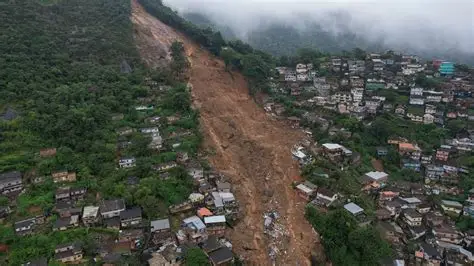
\includegraphics[width=0.8\textwidth]{Images/Brazil.png}}
\only<2>{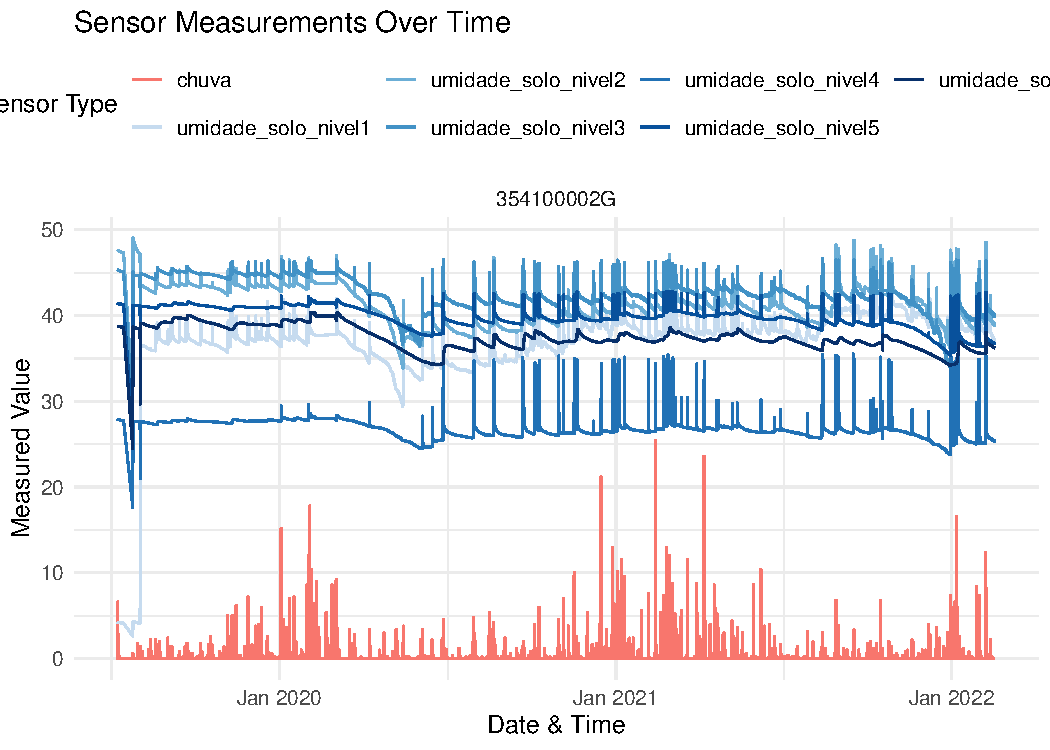
\includegraphics[width=0.8\textwidth]{Images/Plot1.pdf}}
\end{frame}



\begin{frame}
\frametitle{Motivating Example II - Storms across Ireland}
\begin{center}
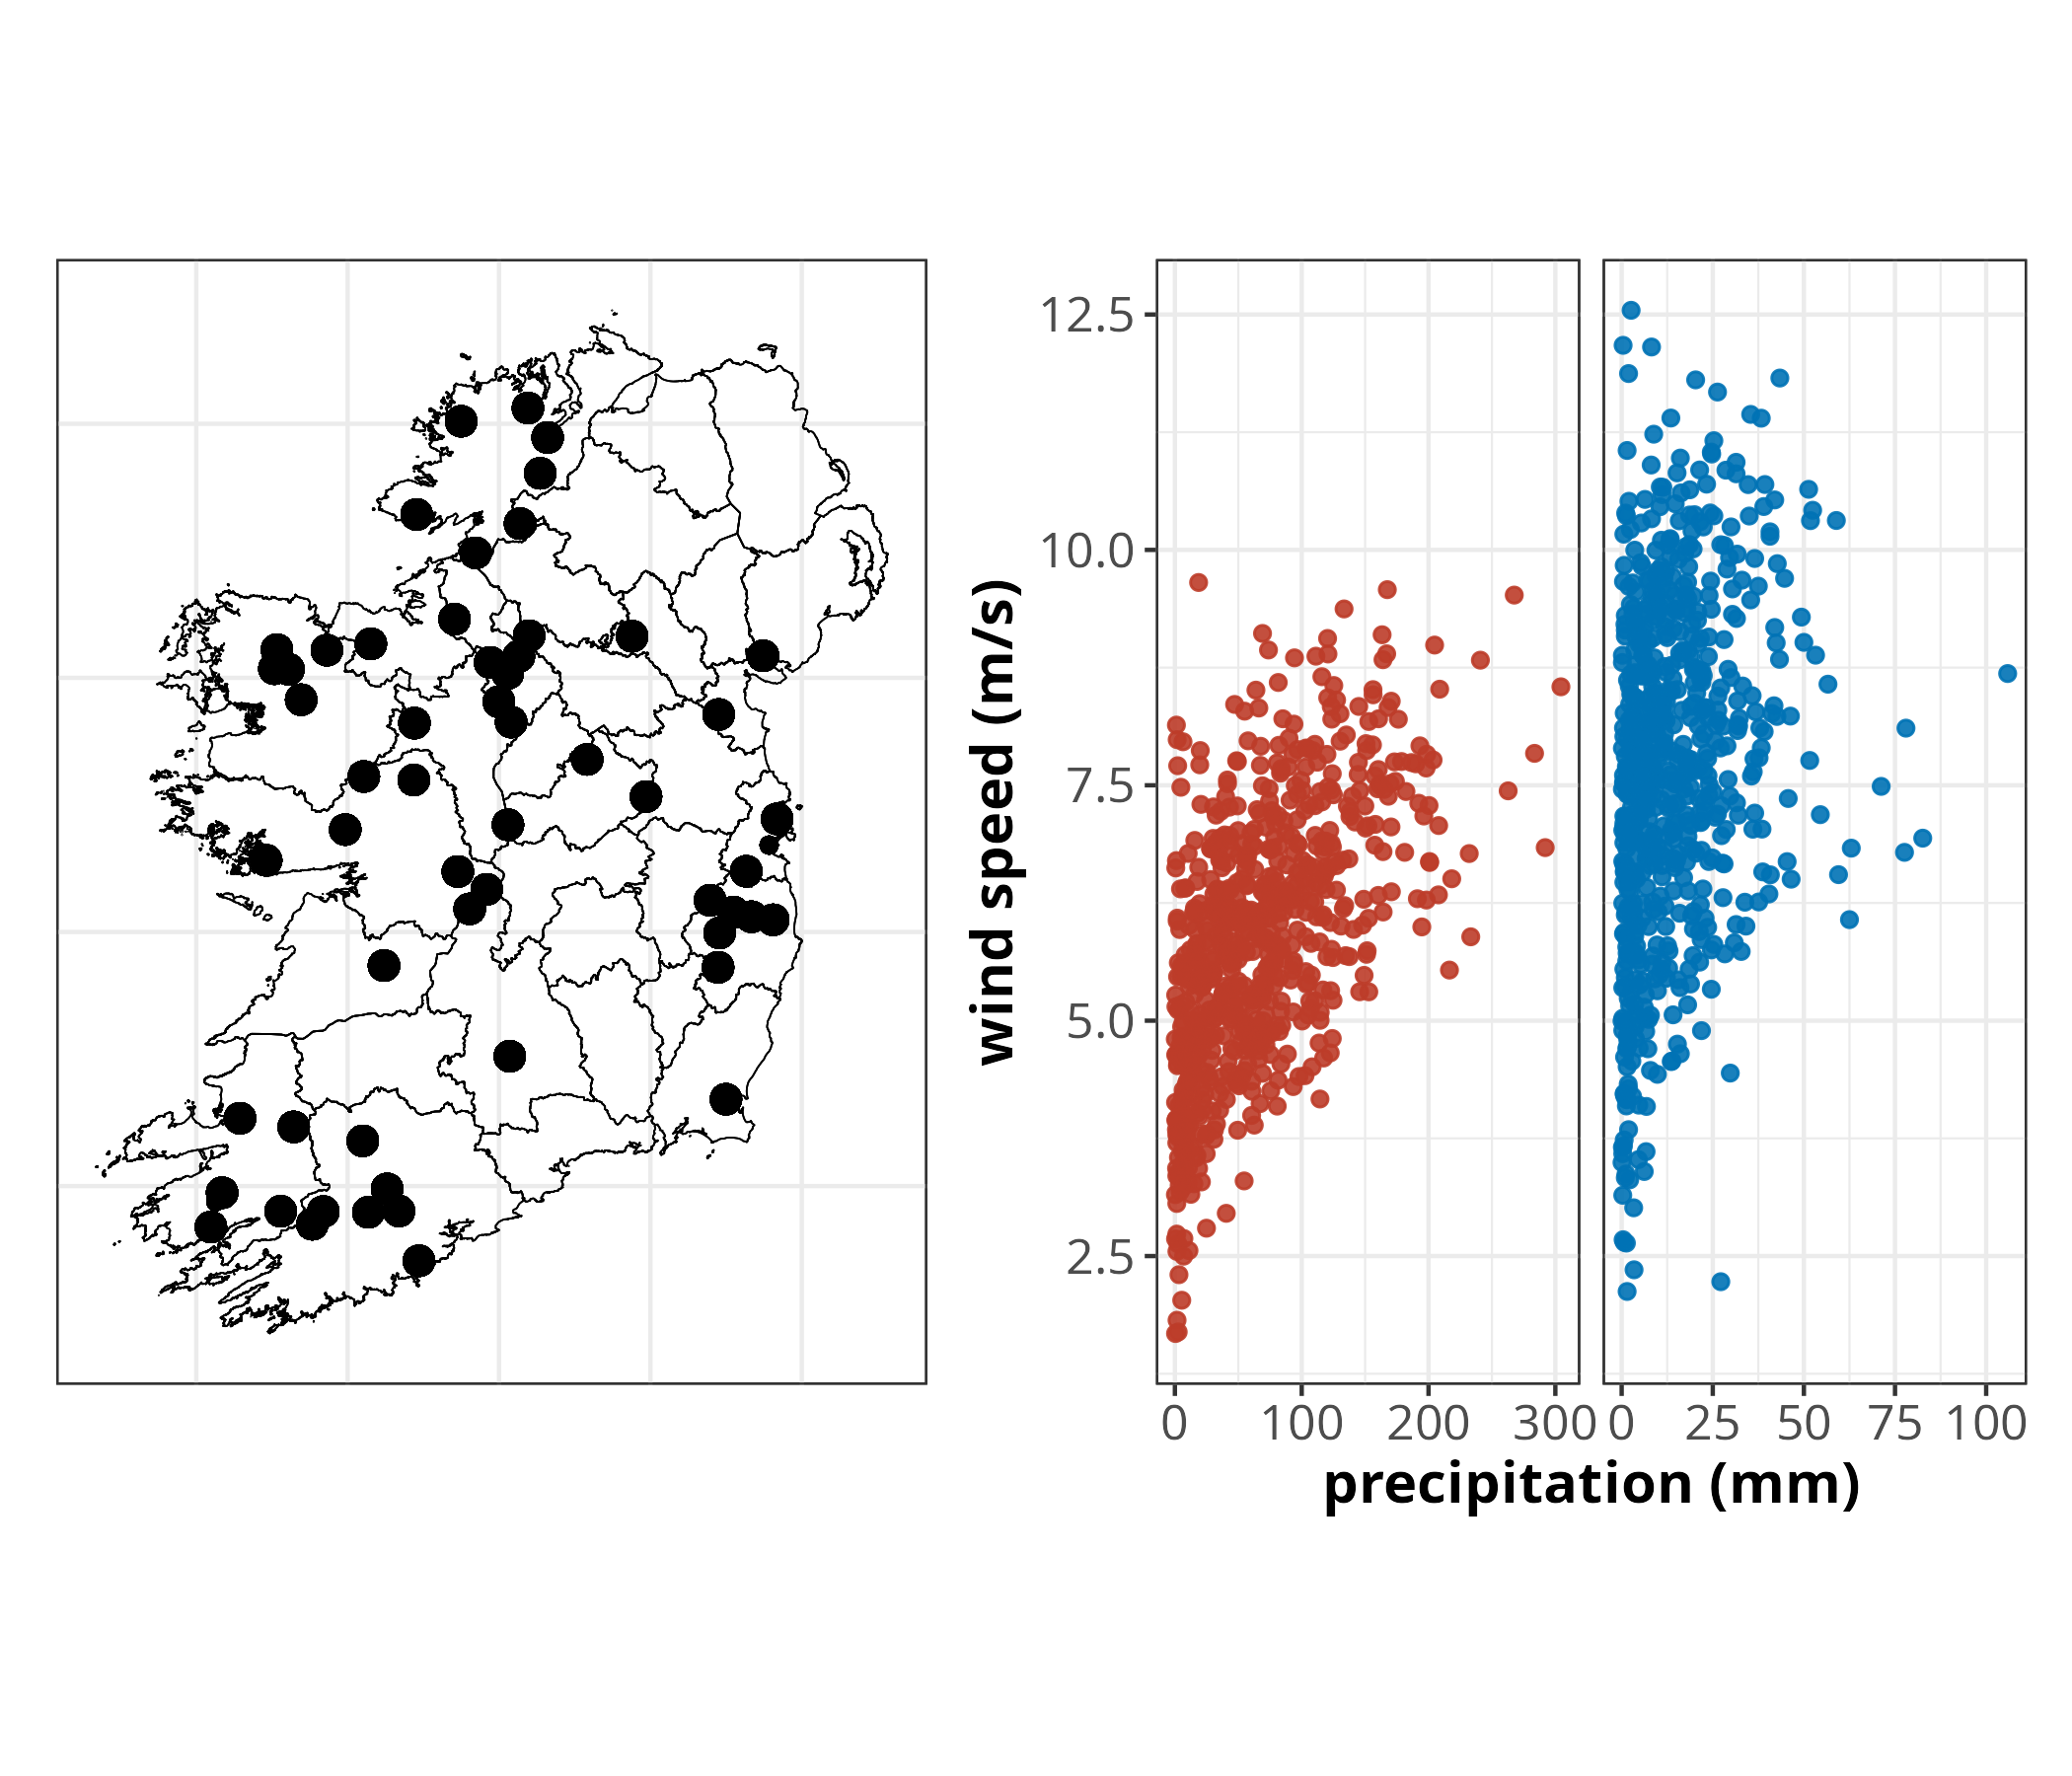
\includegraphics[width=0.9\textwidth]{Images/ire_sites_plt.png}
\end{center}
\end{frame}

\begin{frame}{Background} 
\begin{itemize}
\item Denote $(X,Y) = (\mathrm{Amount~of~Rainfall}, \mathrm{Wind~speed})$.\vspace{0.2cm}
\item One common measure for dependence in the tail of $(X,Y)$ is
\[
\chi = \lim_{u\to 1}  \mathbb{P}\left[F_X(X)>u \mid F_Y(Y) > u \right].
\]
\end{itemize}

\begin{center}
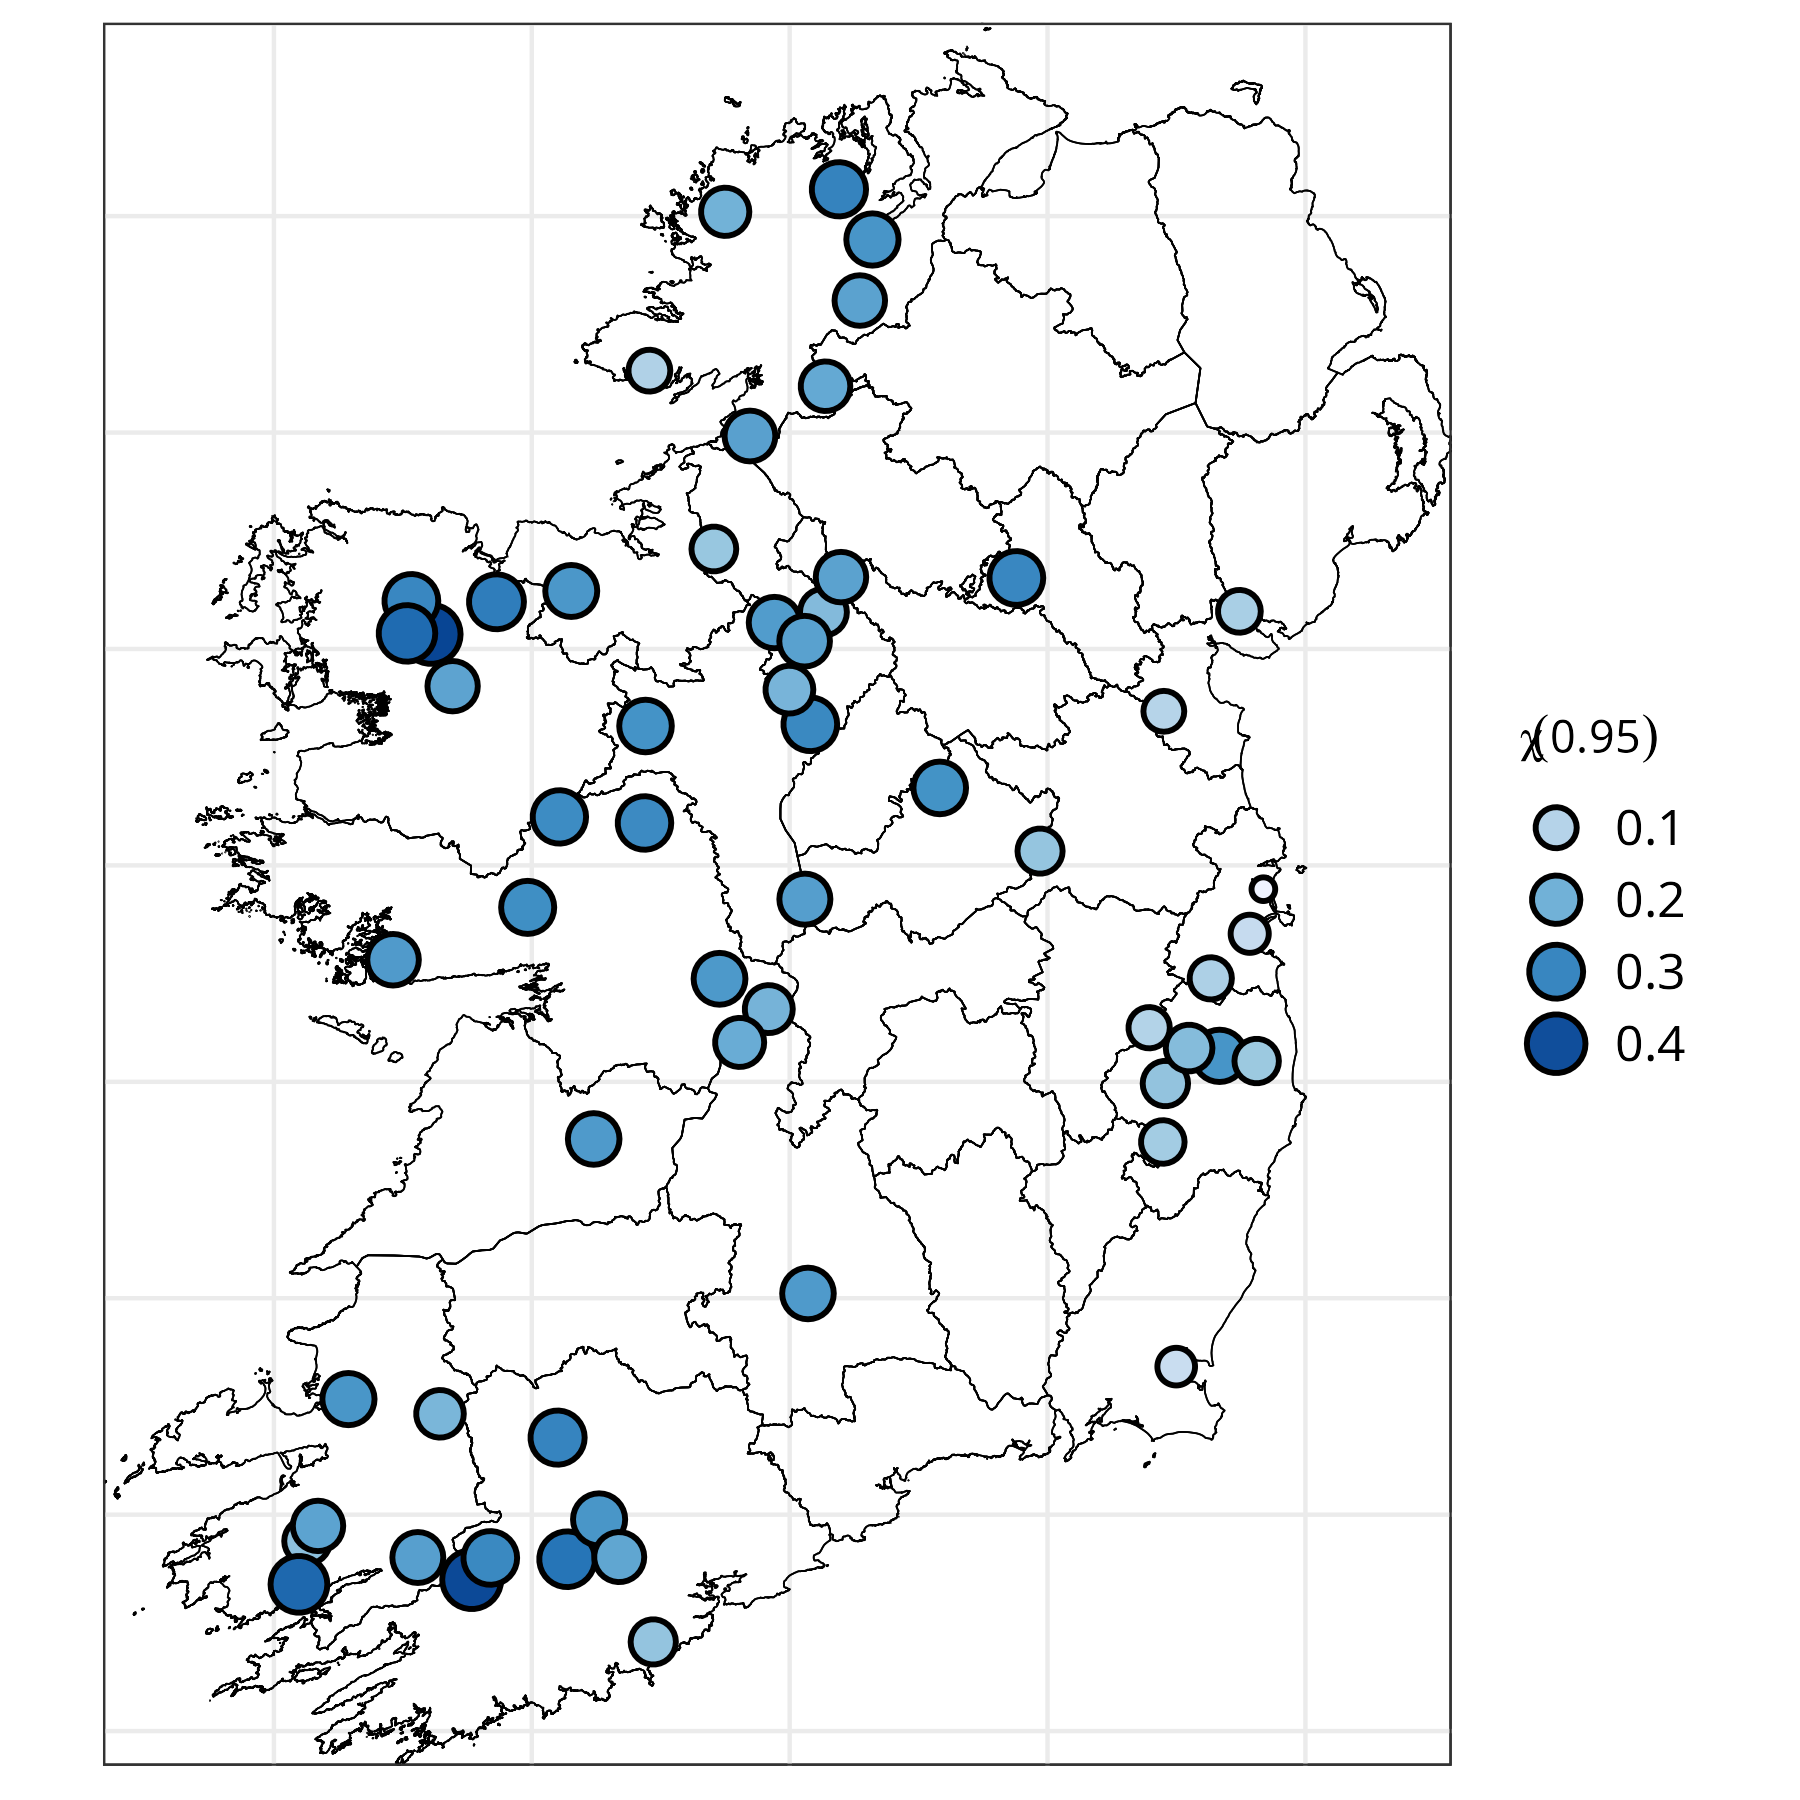
\includegraphics[width=0.45\textwidth]{Images/chi_map_ire.png}
\end{center}
\end{frame}

\begin{frame}
\frametitle{Aims}
\begin{itemize}
\item We find some spatial trend in the estimates for $\chi$.\vspace{0.4cm}
\item \textbf{However:} $\chi$ does not give a full picture of the dependence between rainfall and wind speed.\vspace{0.4cm}
\item Can we identify sites with a similar relation of extreme values?\vspace{0.2cm}\pause
\item \textbf{Our approach:} Identify groups of sites with a similar dependence structure by combining:\vspace{0.2cm}
\begin{enumerate}
\item Conditional extremes models;\vspace{0.2cm}
\item Clustering.
\end{enumerate}
\end{itemize}
\end{frame}

\setbeamertemplate{section page}[mine][]
\section*{Clustering of conditional extremes models}

\begin{frame}
\sectionpage
\end{frame}

\begin{frame}
\frametitle{Conditional extremes models}
We study the distribution of $Y$ conditional on $X$ being large.\vspace{0.2cm}

\textbf{STEP 1:} Transform $X$ and $Y$ to Laplace margins to get $(\tilde{X},\tilde{Y})$.\vspace{0.2cm}
 
\textbf{STEP 2:} Assume that there exists $\alpha$, $\beta$ and $G_x()$ such that
\[
\tilde{Y} = \alpha \tilde{X}  + {\tilde{X}^\beta} Z, 
\]
where $G_x()$ is the distribution of $Z$.\vspace{0.2cm}

\textbf{STEP 3:} Estimate $\alpha$, $\beta$ and $G_x$ from the data. \vspace{0.4cm}\pause

\textbf{Our assumptions:}
\begin{itemize}
\item Residuals $Z \sim \mathrm{Normal}(\mu, \sigma^2)$ 
\item $Z$ is conditionally independent of $\tilde{X}$
\end{itemize}
\end{frame}

\begin{frame}
\frametitle{Illustration - STEP 1}
Using
  \begin{equation} \label{eq:laplace}
    \tilde{X} = \begin{cases}
      \log\left\{2F_{X}(X)\right\} &\text{ for } X < F_{X}^{-1}(0.5), \\
      -\log\left\{2(1 - F_{X}(X))\right\} &\text{ for } X \ge F_{X}^{-1}(0.5), \\
    \end{cases}
  \end{equation}
\begin{center}
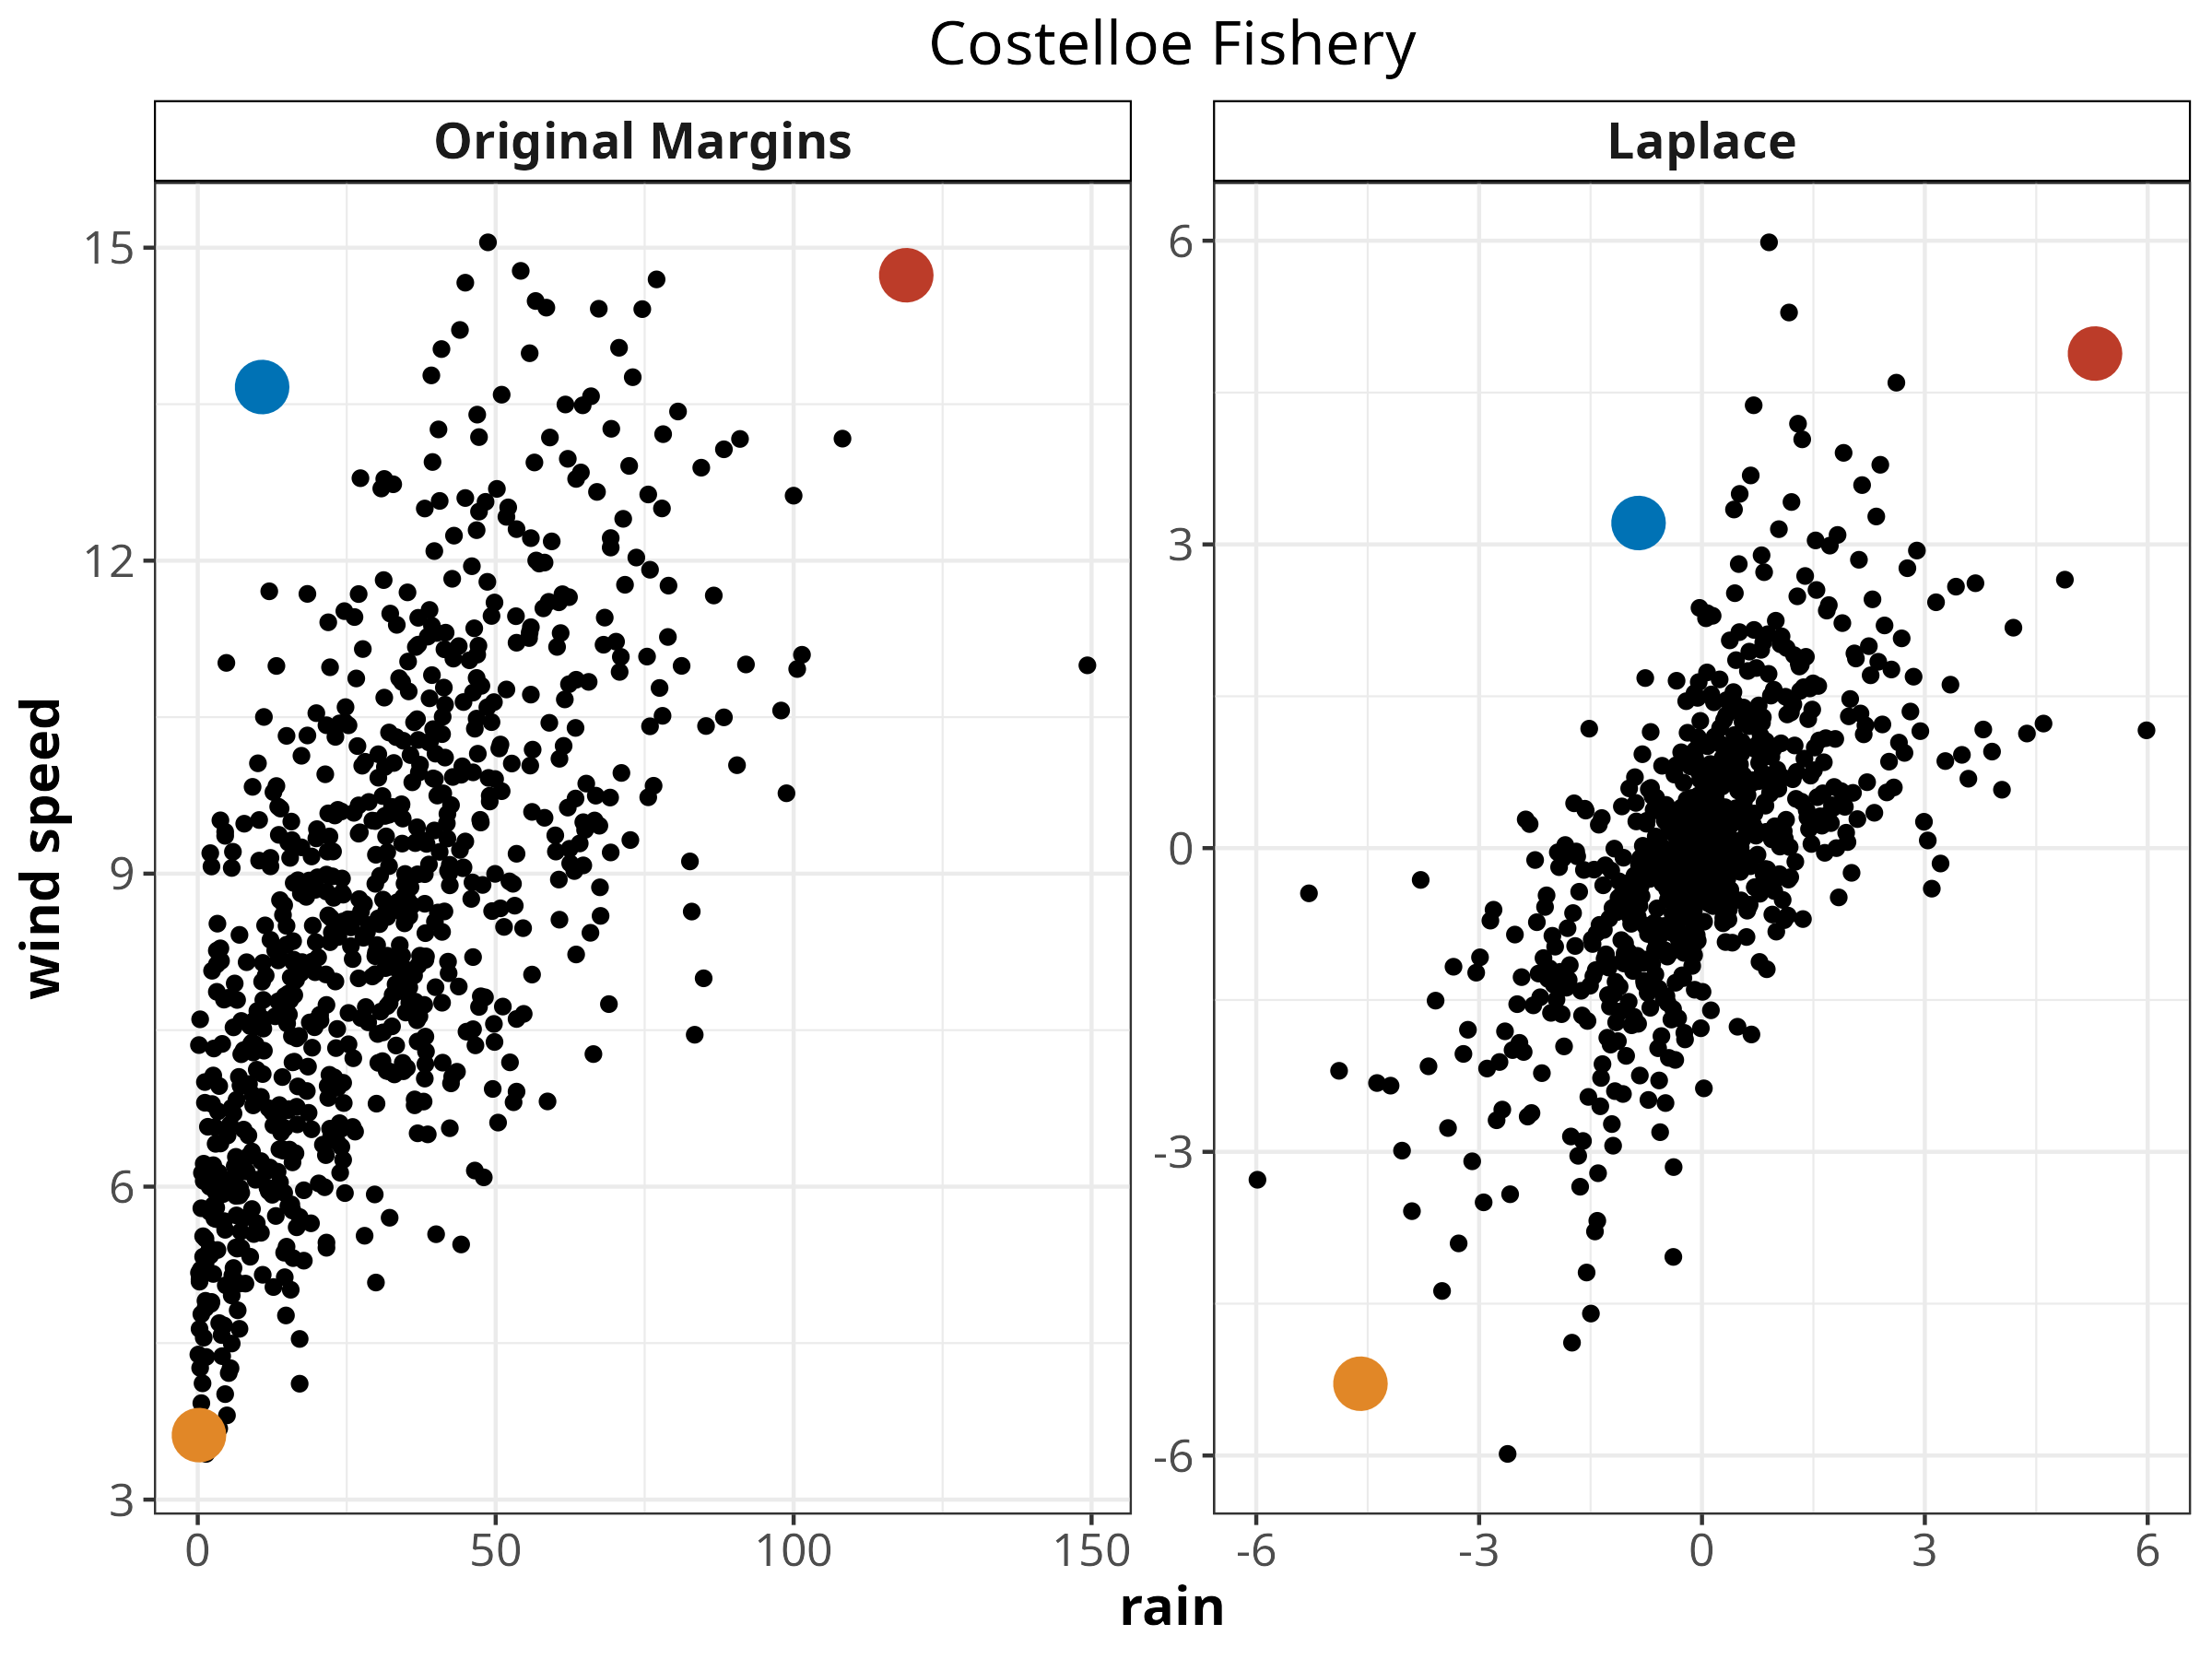
\includegraphics[width=0.55\textwidth]{Images/transformCostelloe.png}
\end{center}
\end{frame}

\begin{frame}
\frametitle{Illustration - STEP 2+3}
\begin{center}
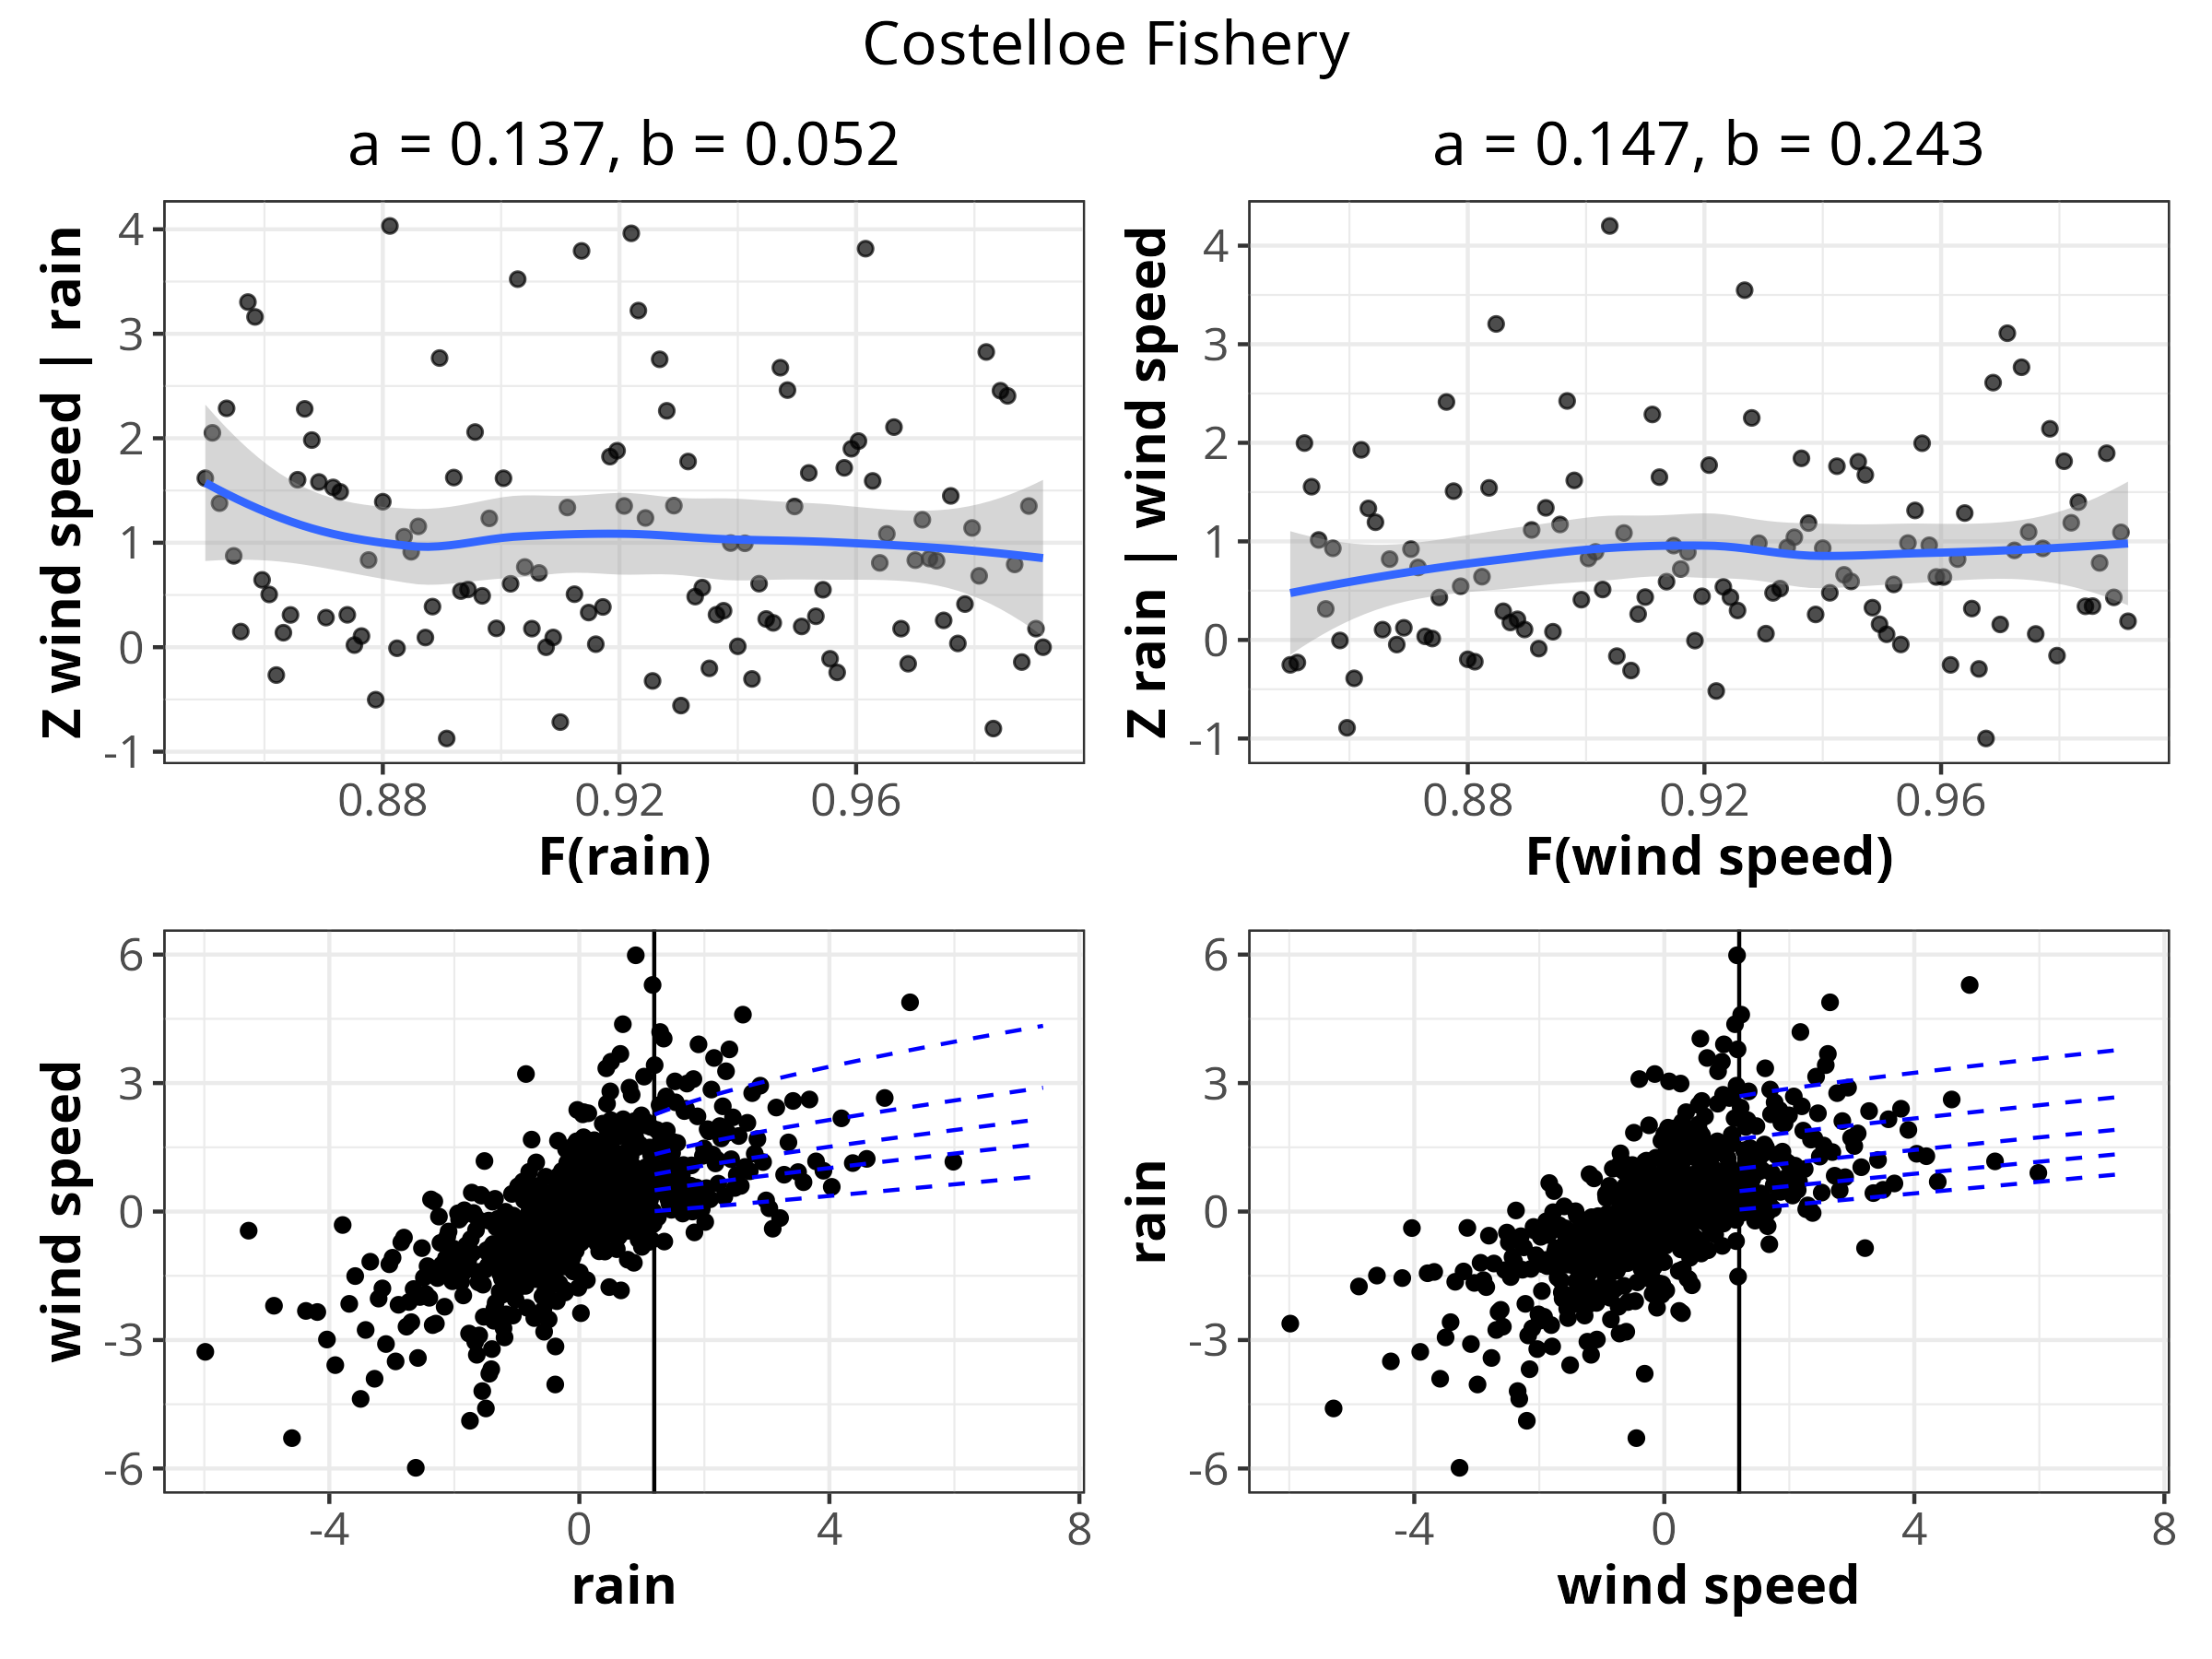
\includegraphics[width=0.7\textwidth]{Images/CostelloeFishery.png}
\end{center}
\end{frame}

\begin{frame}
\frametitle{Measuring similarity of CE models I}
Suppose we have fitted models for $\tilde{Y}(s) \mid \tilde{X}(s)$ for all sites.\vspace{0.4cm}

How do we define a distance between two models? \vspace{0.4cm}\pause

One classical measure is the Kullback-Leibler divergence
\[
KL(P \mid\mid Q) = \int_{-\infty}^{\infty} p(y) \log\left(\frac{p(y)}{q(y)}\right) \mathrm{d}y.
\]
\end{frame}

\begin{frame}
\frametitle{Measuring similarity of CE models II}
We suggest to use the skew-geometric Jensen Shannon divergence
\begin{equation} \label{eq:js_norm}
JS^{G_{\alpha}}(P \mid\mid Q) = \frac{1}{2} KL(P \mid\mid G_{\alpha}(P, Q)) + \frac{1}{2} KL(Q \mid\mid G_{\alpha}(P, Q)),
\end{equation}
with $G_{\alpha}(P, Q) = P^{\alpha} Q^{1 - \alpha}$, and $\alpha \in [0, 1]$.\pause\vspace{0.3cm}

Since the models $P$ and $Q$ depend on the value of $X$, we define the expected value
\[
\int_{u}^\infty JS^{G_{\alpha}}(P(x) \mid\mid Q(x)) f(x) \mathrm{d}x,
\]
where $f(x)$ is the marginal density for $\tilde{X}\mid \tilde{X}>u$.
\end{frame}

\begin{frame}
\frametitle{Clustering}

\begin{enumerate}
\item Fit the conditional extremes models.\vspace{0.3cm}

\item Set the distance between models to the estimate for the expected value:\vspace{0.2cm}
\begin{itemize}
\item Closed-form expression for $JS^{G_{\alpha}}(P(x) \mid\mid Q(x))$ under the assumption of normality.\vspace{0.2cm}
\item Monte Carlo integration to estimate the expected value.\vspace{0.3cm}
\end{itemize}

\item Apply a clustering algorithm of your choice. We choose k-medoids.
\end{enumerate}
\end{frame}

\begin{frame}
\frametitle{Selecting the number of clusters}
We select number of clusters using the Total Within Group Sum of Squares (TWGSS).\vspace{0.3cm}

  \begin{center}
    \vspace{-0.3cm}
    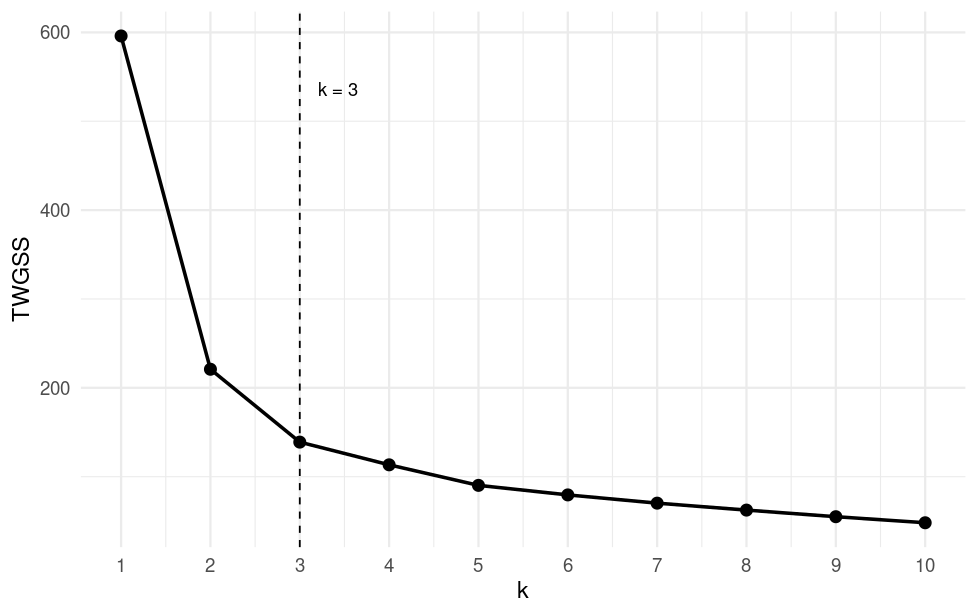
\includegraphics[width=0.6\textwidth]{Images/elbow_plot.png}
  \end{center}
\end{frame}


\setbeamertemplate{section page}[mine][]
\section*{Simulation Studies}

\begin{frame}
\sectionpage
\end{frame}

\begin{frame}
\frametitle{Study 1 - Gaussian Copula}
\begin{itemize}
    \item For single ``site'', generate data from bivariate Gaussian copula with correlation $\rho$.\vspace{0.3cm}
    \item Conditional extremes parameters are $\alpha = \rho^2$ and $\beta = 1/2$.\vspace{0.3cm}
    \item We sample 12 ``sites'' with 10000 observations for 2 variables.\vspace{0.3cm}
    \item 3 clusters of 4 locations defined by respective $\rho$ values of $0.1, 0.5, 0.9$.
  \end{itemize}
\end{frame}	

\begin{frame}{Results}
  \center
  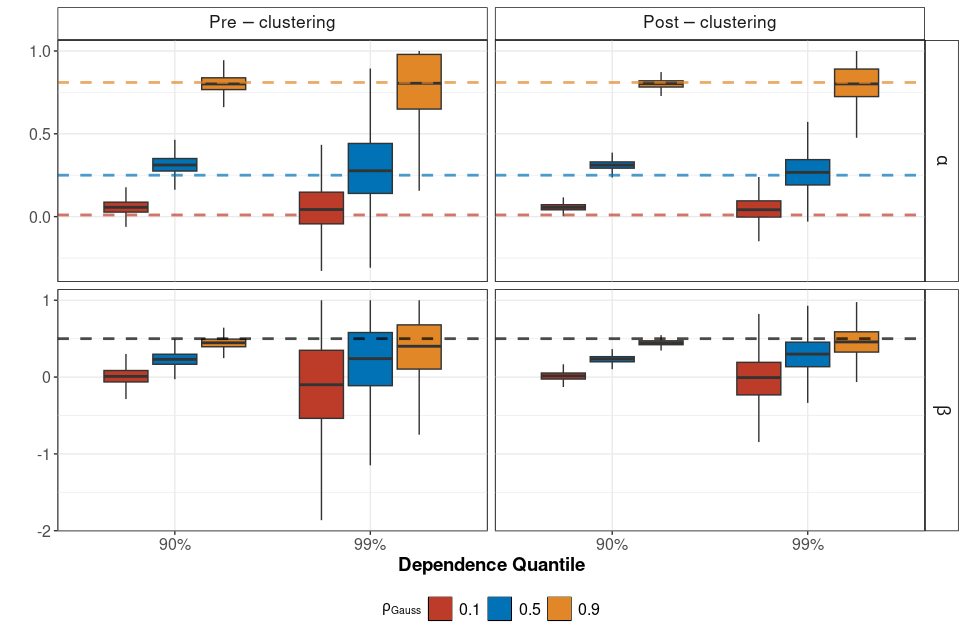
\includegraphics[width=\textwidth]{Images/sim_01_gauss_cop_man.png}
\end{frame}
	
\begin{frame}{Study 2 - Mixture model}
\begin{itemize}
\item Extend design to mixture of Gaussian and t-copulas: \vspace{0.3cm}
    \begin{itemize} 
      \item Gaussian copula generates observations exhibiting extremal independence,\vspace{0.2cm} 
      \item t-copula induces extremal dependence.
    \end{itemize}
\item 12 sites with 10000 bivariate observations.\vspace{0.3cm}
\item 2 clusters of 6 sites.\vspace{0.3cm}
\item Grid search performed over $\rho, \rho_{t_1}, \rho_{t_2} \in [0, 1]$.\vspace{0.3cm}
\item Clustering compared to Vignotto (2021) algorithm using Adjusted Rand Index $\text{ARI} \in [0, 1]$ 
\end{itemize}
\end{frame}	

\begin{frame}{Results}
  \center
  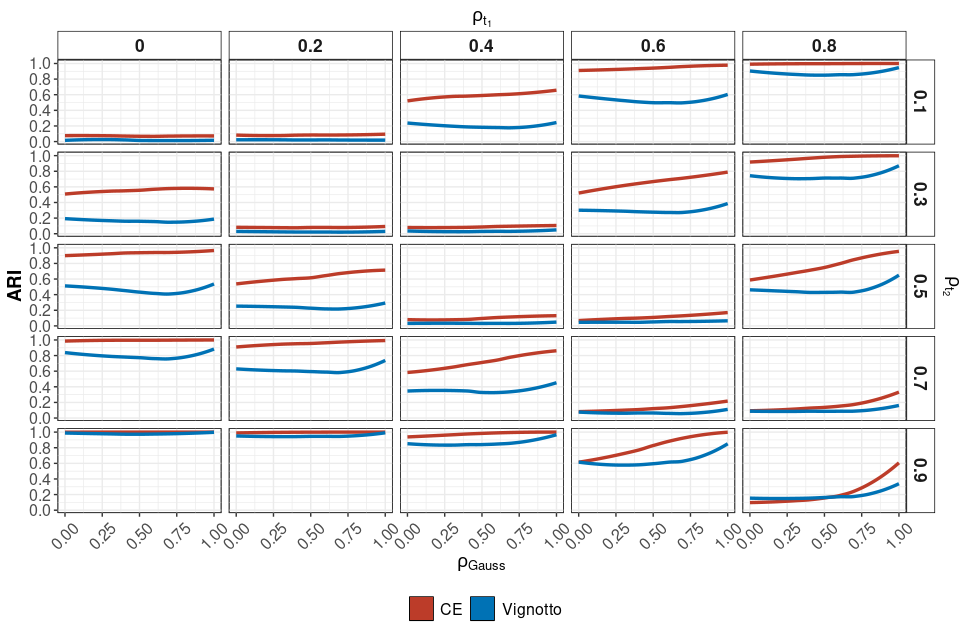
\includegraphics[width=1\textwidth]{Images/sim_01b_ce_vs_vi_dqu_0.9_man.png}
\end{frame}


\section{Case Study}

\begin{frame}
\sectionpage
\end{frame}

\begin{frame}
\frametitle{Setup}
\begin{itemize}
\item Slightly more than 50 sites from 20 counties.\vspace{0.3cm}
\item Data for 1990-01-01 to 2020-12-31.\vspace{0.3cm}
\item Weekly sum of precipitation and averages of wind speed maxima.\vspace{0.3cm}
\item We consider the period November to March only.
\end{itemize}
\end{frame}

\begin{frame}{Results for Ireland}
\center
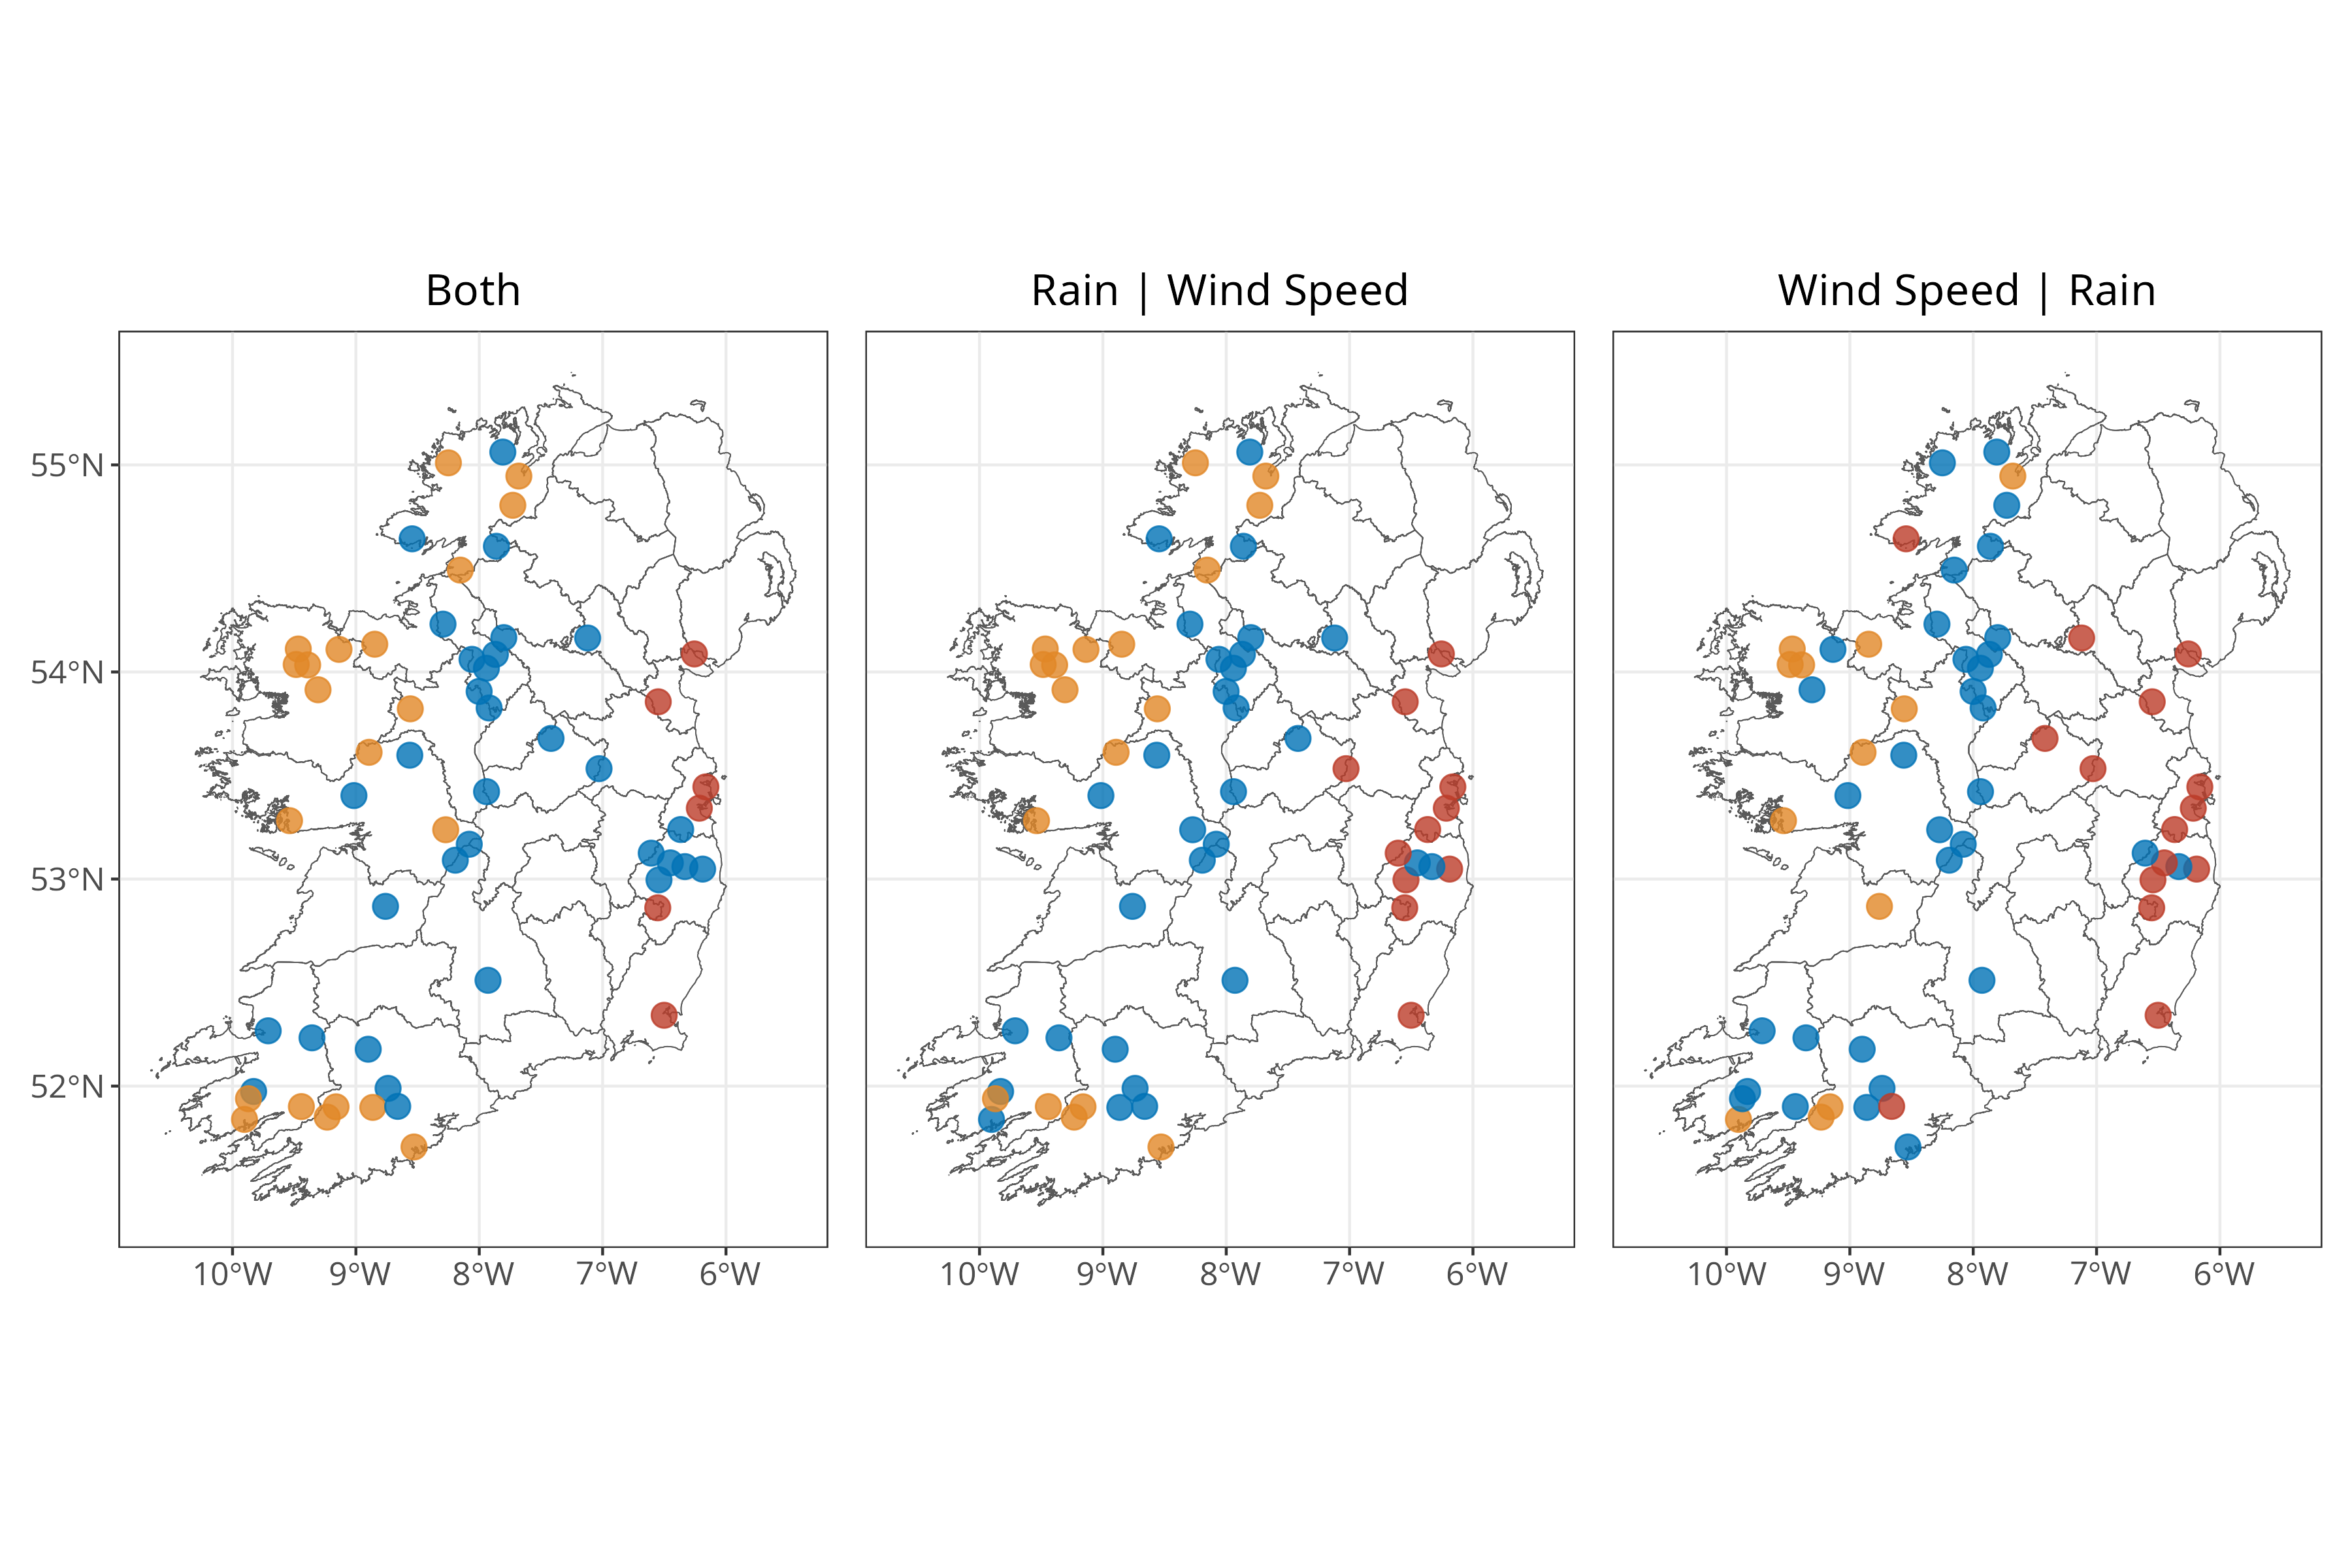
\includegraphics[width=0.9\textwidth]{Images/cluster_dqu_sep.png} 
\end{frame}

\begin{frame}{Discussion}
  \begin{itemize}
    \item <1-> \textbf{Conclusion}:\vspace{0.2cm}
      \begin{itemize}
        \item Principled \& effective clustering framework for CE models\vspace{0.2cm}
        \item We identify group sites with similar tail dependence\vspace{0.2cm}
				\item Computationally efficient\vspace{0.4cm}
      \end{itemize} 
    \vspace{2mm}
    \item <2-> \textbf{Limitations}:\vspace{0.2cm}
      \begin{itemize}
        \item Gaussian assumption for $Z$\vspace{0.2cm}
        \item Uncertainty in model fits has been ignored\vspace{0.4cm}
      \end{itemize} 
		\item <3-> \textbf{Paper and R software package to come soon!}	
  \end{itemize}
\end{frame}	

\begin{frame}
\frametitle{References}

\begin{thebibliography}{10}    
\small
\bibitem{C1} Keef, C, Papastathopoulos, I \& Tawn, JA. \textit{Estimation of the conditional distribution of a multivariate variable given that one of its components is large: Additional constraints for the Heffernan and Tawn model}. \textbf{Journal of Multivariate Analysis}, 115, pp.~396-404.

\bibitem{C2} Nielsen, F. \textit{On the Jensen–Shannon Symmetrization of Distances Relying on Abstract Means}. \textbf{Entropy}, 21, 485.\vspace{0.5cm}
\end{thebibliography}

\centering
\huge Thanks a lot for your attention!

\end{frame}
	
\end{document}